% ============================================================
%   CryptoCore-16 Academic Report
%   Compiled with: pdflatex CryptoCore16_Report.tex
%   Required packages: geometry, graphicx, listings, booktabs,
%                      hyperref, fancyhdr, titlesec, xcolor,
%                      amsmath, array, caption, float
% ============================================================

\documentclass[12pt, a4paper]{report}

% ---------- Packages ----------
\usepackage[top=2.5cm, bottom=2.5cm, left=3cm, right=2.5cm]{geometry}
\usepackage{graphicx}
\usepackage{listings}
\usepackage{booktabs}
\usepackage{hyperref}
\usepackage{fancyhdr}
\usepackage{titlesec}
\usepackage{xcolor}
\usepackage{amsmath}
\usepackage{amssymb}
\usepackage{array}
\usepackage{caption}
\usepackage{float}
\usepackage{setspace}
\usepackage{parskip}
\usepackage{enumitem}
\usepackage{multirow}
\usepackage{tabularx}
\usepackage{tcolorbox}
\usepackage{xurl}
\usepackage{tikz}
\usetikzlibrary{arrows.meta, positioning, fit, backgrounds}
\usepackage{xcolor}
\usepackage{float}
\usepackage{tocloft}
\usepackage{titletoc}

\setcounter{tocdepth}{2}
\renewcommand{\cftchapfont}{\bfseries}
\renewcommand{\cftchappagefont}{\bfseries}
\renewcommand{\cftchapaftersnum}{.}
\setlength{\cftbeforechapskip}{8pt}
\setlength{\cftbeforesecskip}{2pt}
\setlength{\cftbeforesubsecskip}{1pt}
\renewcommand{\cftchapleader}{\cftdotfill{\cftdotsep}}


% ---------- VHDL listing style ----------
\definecolor{vhdlblue}{rgb}{0.13,0.13,0.7}
\definecolor{vhdlgreen}{rgb}{0.0,0.5,0.0}
\definecolor{vhdlgray}{rgb}{0.5,0.5,0.5}
\definecolor{vhdlbg}{rgb}{0.97,0.97,0.97}
\definecolor{clkcolor}{RGB}{44,62,80}
\definecolor{regcolor}{RGB}{41,128,185}
\definecolor{alucolor}{RGB}{39,174,96}
\definecolor{shiftcolor}{RGB}{211,84,0}
\definecolor{lutcolor}{RGB}{142,68,173}
\definecolor{muxcolor}{RGB}{192,57,43}
\definecolor{pipecolor}{RGB}{100,110,120}

\lstdefinelanguage{VHDL}{
  morekeywords={library, use, entity, port, in, out, is, end, architecture,
                signal, begin, process, if, then, else, elsif, case, when,
                others, rising_edge, std_logic_vector, std_logic, all,
                downto, to, type, array, of, and, or, not, xor, nor, nand,
                unsigned, integer, block, select, with},
  sensitive=false,
  morecomment=[l]{--},
  morestring=[b]"
}

\lstset{
  language=VHDL,
  basicstyle=\ttfamily\small,
  keywordstyle=\color{vhdlblue}\bfseries,
  commentstyle=\color{vhdlgreen}\itshape,
  stringstyle=\color{red},
  numbers=left,
  numberstyle=\tiny\color{vhdlgray},
  stepnumber=1,
  numbersep=8pt,
  backgroundcolor=\color{vhdlbg},
  showspaces=false,
  showstringspaces=false,
  breaklines=true,
  frame=single,
  rulecolor=\color{black!30},
  tabsize=4,
  captionpos=b
}

% ---------- Header / Footer ----------
\pagestyle{fancy}
\fancyhf{}
\fancyhead[L]{\small CryptoCore-16: 16-bit Cryptographic Coprocessor}
\fancyhead[R]{\small Hardware Design Project}
\fancyfoot[C]{\thepage}
\renewcommand{\headrulewidth}{0.4pt}
\setlength{\headheight}{14pt}

% ---------- Layout helpers ----------
\setlength{\emergencystretch}{3em}
\newcolumntype{Y}{>{\raggedright\arraybackslash}X}

% ---------- Spacing ----------
\onehalfspacing

% ---------- Chapter title format ----------
\titleformat{\chapter}[block]
  {\normalfont\LARGE\bfseries}
  {\thechapter.}{1em}{}
\titlespacing*{\chapter}{0pt}{20pt}{15pt}

% ---------- Hyperref setup ----------
\hypersetup{
  colorlinks=true,
  linkcolor=blue!70!black,
  citecolor=green!50!black,
  urlcolor=blue
}


% ============================================================
%   DOCUMENT BEGIN
% ============================================================
\begin{document}

% ============================================================
%   COVER PAGE
% ============================================================
\hypersetup{pageanchor=false}
\begin{titlepage}
\centering

\vspace*{1cm}

% University / Department logo placeholder
% ----------------------------------------------------------------
% [INSERT UNIVERSITY LOGO HERE]
% \includegraphics[width=0.35\textwidth]{university_logo.png}
% ----------------------------------------------------------------

\vspace{1cm}



{\Huge \textbf{CryptoCore-16}}\\[0.4cm]
{\Large \textbf{16-bit Cryptographic Coprocessor Design in VHDL}}\\[0.3cm]
\noindent\rule{\linewidth}{1.5pt}

\vspace{1.2cm}

\begin{tcolorbox}[colback=gray!10, colframe=gray!50, width=0.85\textwidth]
  \centering
  {\large \textbf{Course:} Hardware Design and Digital Systems}\\[0.3cm]
  {\large  Under supervision of professor \textbf{Howaida Abdul Latif}} \\[0.3cm]
\end{tcolorbox}

\vspace{1.5cm}

{\large \textbf{Submitted by:}}\\[0.5cm]

{\footnotesize
\setlength{\tabcolsep}{5pt}
\renewcommand{\arraystretch}{1.2}
\noindent\makebox[\textwidth][c]{%
\begin{tabularx}{1.18\textwidth}{>{\raggedright\arraybackslash}p{3.8cm}p{3.4cm}Y Y}
  \toprule
  \textbf{Name} & \textbf{Student ID} & \textbf{Email} & \textbf{Work} \\
  \midrule
  Hatem Ayman Nabil & 20812023100716 & \nolinkurl{hatem.ayman.508@gmail.com} & Project coordination and testing, combinational logic block \\
  Amal Ragab El-Muhammady & 20812023200455 & \nolinkurl{ragabaml242@gmail.com} & Register, \texttt{crypto\_core16 TB} \\
  Alsayed Abdul Raouf Ahmed & 20812023100463 & \nolinkurl{elsayed2005920@gmail.com} & Nonlinear lookup table, \texttt{Crypto\_core16} \\
  Alaa Muhammad Thabet & 20812023200555 & \nolinkurl{am5897667@gmail.com} & Shifter unit / shifter TB \\
  Eyad Islam El-Taher & 20812023100040 & \nolinkurl{eltahereyad0@gmail.com} & ALU \& ALU TB \& Report \\
  \bottomrule
\end{tabularx}%
}
}

\vfill


\end{titlepage}

\clearpage
\hypersetup{pageanchor=true}
\pagenumbering{arabic}

% ============================================================
%   TABLE OF CONTENTS
% ============================================================
\clearpage
{
  \hypersetup{linkcolor=black}
  \renewcommand{\contentsname}{Table of Contents}
  \tableofcontents
}
\newpage

% ============================================================
\chapter{Assignment Aim}
% ============================================================

The primary objective of this project is to design, implement, and verify a
\textbf{16-bit Cryptographic Coprocessor} (CryptoCore-16) using VHDL (VHSIC Hardware Description Language).
The coprocessor is intended to accelerate computationally intensive cryptographic operations
that would otherwise be a bottleneck for a general-purpose central processing unit (CPU).

Specifically, the project aims to:

\begin{enumerate}[label=\arabic*.]
  \item Design a complete hardware architecture capable of executing a defined set of 12
        cryptographic and arithmetic instructions.
  \item Implement a modular VHDL design consisting of five major components:
        an Input Pipeline Register, a 16$\times$16 Register File, an Arithmetic Logic Unit (ALU),
        a Shifter Unit, and a Non-Linear Lookup Table (LUT / S-Box).
  \item Integrate all components into a single top-level entity (\texttt{crypto\_core16})
        that orchestrates data flow and control.
  \item Validate the correctness of each component independently through dedicated VHDL
        testbenches, and verify the full system behaviour through integration simulation.
  \item Demonstrate how hardware-level parallelism and pipelining improve the throughput
        and latency of cryptographic operations compared to equivalent software implementations.
\end{enumerate}

The design follows a \textbf{Register–Execute–Write-back} pipeline model where all components
operate in a coordinated manner, governed by a 4-bit control signal (\texttt{CTRL}) that encodes
the instruction opcode. The implementation tool used for simulation is
\textbf{Aldec Active-HDL}, and all source files are written in synthesisable VHDL-93 / VHDL-2008.

% ============================================================
\chapter{The Problem and Solution}
% ============================================================

\section{Problem Description}

\subsection{The Need for a Cryptographic Coprocessor}

Modern digital systems, spanning from Internet-of-Things (IoT) devices to enterprise servers,
must protect data in transit and at rest against a broad range of adversarial threats.
Cryptographic algorithms—such as the Advanced Encryption Standard (AES), Data Encryption
Standard (DES), and elliptic-curve cryptography (ECC)—provide the mathematical foundation
for this protection. However, executing these algorithms entirely in software on a
general-purpose CPU presents several serious drawbacks \cite{tan2021hardware}.

A software cryptographic implementation consumes a substantial fraction of the CPU's
processing cycles. Every XOR, substitution table lookup, rotation, and modular addition
that constitutes a cryptographic round must be performed sequentially by the CPU's
instruction pipeline. For algorithms such as AES-128, a single encryption block requires
10 rounds, each involving four distinct transformations (SubBytes, ShiftRows, MixColumns,
AddRoundKey), applied to 128 bits of data. When a system must handle thousands of encrypted
connections simultaneously—as in a web server or a wireless base station—this sequential
execution model becomes a severe throughput bottleneck \cite{nassim2025fpga}.

Beyond raw throughput, software implementations are also vulnerable to \textbf{timing attacks}:
a class of side-channel attack in which an adversary deduces secret key material by
measuring subtle variations in the execution time of cryptographic operations. Because
software runs on shared hardware resources (caches, branch predictors, memory buses),
the time required to compute a substitution or an inversion in $\mathrm{GF}(2^8)$ may
vary with the input value, inadvertently leaking information \cite{nassim2025fpga}.

\subsection{Challenges in Hardware-Based Cryptography}

Implementing cryptography in hardware introduces its own set of engineering challenges:

\begin{enumerate}[label=\arabic*.]
  \item \textbf{Non-linear transformations:} The S-Box (substitution box) is the primary
        source of non-linearity in block ciphers. Computing the multiplicative inverse in
        the finite field $\mathrm{GF}(2^8)$ followed by an affine transformation is
        expensive to implement efficiently in combinational logic.

  \item \textbf{Instruction-level resource sharing:} A crypto coprocessor must support
        multiple operation classes (arithmetic, bitwise logic, rotation, and substitution)
        using a single unified data path, requiring careful multiplexing and control logic.

  \item \textbf{Timing and pipeline hazards:} Registering inputs before feeding them to
        combinational logic avoids glitches and ensures stable operation across clock
        domains, but introduces pipeline latency that must be accounted for.

  \item \textbf{Write-back control:} Not all instructions should modify the register file
        (e.g., NOP). The write-enable signal must be generated correctly to prevent
        unintended state corruption.

  \item \textbf{Simulation and verification:} Each functional block must be independently
        verified before integration, necessitating comprehensive testbenches that cover
        boundary conditions and all opcode combinations.
\end{enumerate}

\section{Proposed Solution}

\subsection{System Architecture and Approach}

CryptoCore-16 addresses the challenges described above through a \textbf{modular,
fully synthesisable VHDL architecture} organised into five hierarchical layers,
assembled into a single top-level entity. The design philosophy is:

\begin{itemize}
  \item \textbf{Separation of concerns:} Each functional unit (ALU, Shifter, LUT) is
        implemented as a self-contained VHDL entity with well-defined ports.
        The combinational logic block instantiates all three units structurally and
        selects the correct output through a CTRL-driven multiplexer.

  \item \textbf{Parallel execution:} All three functional units (ALU, Shifter, LUT)
        compute their results simultaneously in parallel for every clock cycle.
        The control multiplexer then routes only the relevant result to the output.
        This parallelism mirrors the approach used in high-performance FPGA
        implementations \cite{nassim2025fpga}.

  \item \textbf{Constant-time operation:} The LUT-based S-Box substitution executes in a
        single combinational evaluation—independent of the input value—eliminating the
        timing variations that enable side-channel attacks.

  \item \textbf{Pipeline register:} A single-stage input register captures the opcode
        and register addresses on the rising clock edge, providing a clean, glitch-free
        control environment for the combinational logic below it.

  \item \textbf{Unified Instruction Set Architecture (ISA):} A 4-bit opcode (\texttt{CTRL})
        encodes 12 distinct instructions distributed across the three functional units,
        enabling a compact instruction format: $[\,\text{CTRL}_{3:0}\;|\;\text{Ra}_{3:0}\;|\;\text{Rb}_{3:0}\;|\;\text{Rd}_{3:0}\,]$.
\end{itemize}

The overall data flow is: external control signals enter the \textbf{Input Pipeline Register}
$\rightarrow$ the \textbf{Register File} reads two source operands onto ABUS and BBUS
$\rightarrow$ the \textbf{Combinational Logic Block} computes the result
$\rightarrow$ the result is written back to the destination register \texttt{Rd}
on the next rising clock edge, subject to write-enable gating.

% ============================================================
\chapter{Implementation}
% ============================================================

\section{System Architecture}

The CryptoCore-16 architecture is composed of six distinct VHDL entities,
each residing in its own source file. Figure~\ref{fig:top_block} shows the top-level
block diagram of the system.

% ----------------------------------------------------------------
% [INSERT FIGURE: Top-level block diagram of CryptoCore-16]
% Caption: Figure 5.1 — Top-level architecture of CryptoCore-16.
% The diagram should show: clock, reset, CTRL, Ra, Rb, Rd as inputs;
% the Input Pipeline Register feeding ctrl_tmp and RdWEn;
% the Register File producing ABUS and BBUS;
% the Combinational Logic Block consuming ABUS, BBUS, ctrl_tmp
% and producing RESULT; and the write-back path from RESULT to the Register File.
% (Export this from Active-HDL as a schematic screenshot)
% ----------------------------------------------------------------

\begin{figure}[H]
  \centering
  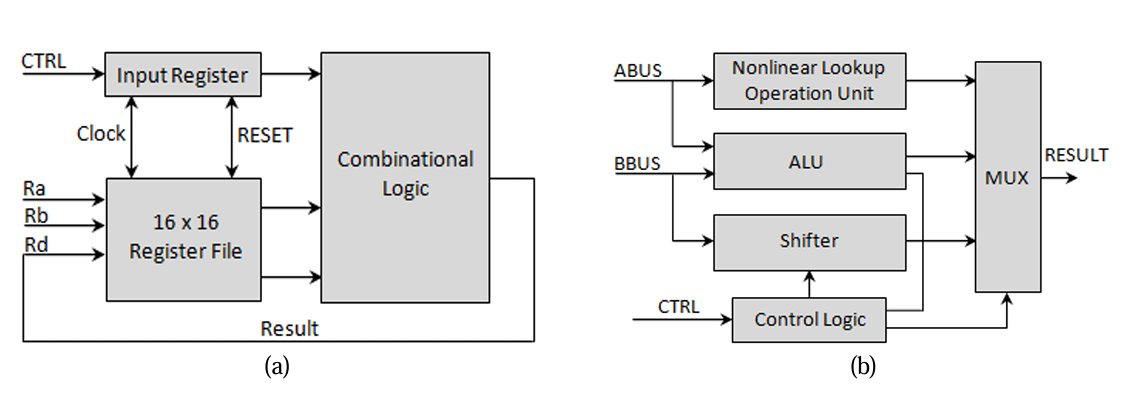
\includegraphics[width=0.9\textwidth]{top level block diagram.png}
  \vspace{0.5cm}
  \caption{Top-level block diagram of CryptoCore-16.}
  \label{fig:top_block}
\end{figure}

\subsection{Input Register (Pipeline Stage)}

The Input Register is not a separate VHDL entity but is implemented as the
\texttt{Process\_control} process inside the top-level \texttt{crypto\_core16} entity.
Its role is to register the external control inputs—specifically \texttt{CTRL}—on
every rising edge of \texttt{clock} before passing them to the combinational logic block.

The process performs two tasks simultaneously:
\begin{itemize}
  \item It registers the incoming \texttt{CTRL} opcode into an internal signal
        \texttt{ctrl\_tmp}, isolating the combinational logic from glitches on the
        primary input.
  \item It generates the write-enable signal \texttt{RdWEn}: this signal is asserted
        high for every instruction \emph{except} NOP (\texttt{"0111"}), preventing
        spurious writes to the register file during idle cycles.
\end{itemize}

\newpage
On a synchronous reset, \texttt{ctrl\_tmp} is forced to \texttt{"0111"} (NOP) and
\texttt{RdWEn} is de-asserted, ensuring the system starts in a safe, quiescent state.

% ----------------------------------------------------------------
% [INSERT CODE SNIPPET: Process_control process from crypto_core16.vhd]
% Show the rising_edge process that registers ctrl_tmp and generates RdWEn.
% Highlight the NOP check: if CTRL = "0111" then RdWEn <= '0'.
% ----------------------------------------------------------------

\begin{lstlisting}[caption={Input pipeline register and write-enable logic (crypto\_core16.vhd).},
                   label={lst:pipeline}]
Process_control : process(clock)
begin
    if rising_edge(clock) then
        if reset = '1' then
            ctrl_tmp <= "0111";   -- Force NOP on reset
            RdWEn    <= '0';      -- Disable write on reset
        else
            ctrl_tmp <= CTRL;     -- Register the opcode

            if CTRL = "0111" then
                RdWEn <= '0';     -- NOP: suppress write-back
            else
                RdWEn <= '1';     -- All other ops: enable write-back
            end if;
        end if;
    end if;
end process;
\end{lstlisting}

\subsection{Register File (16x16)}

The Register File (\texttt{register.vhd}) is the primary working storage of the
coprocessor. It provides:

\begin{itemize}
  \item \textbf{16 registers}, each \textbf{16 bits} wide, modelled as a
        VHDL array \texttt{mem\_type} of 16 elements of type
        \texttt{std\_logic\_vector(15 downto 0)}.
  \item \textbf{Two asynchronous read ports:} reading address \texttt{Ra} drives
        \texttt{SRCa} (mapped to \texttt{ABUS} at the top level), and reading address
        \texttt{Rb} drives \texttt{SRCb} (mapped to \texttt{BBUS}).
        Asynchronous reads introduce zero pipeline latency.
  \item \textbf{One synchronous write port:} on every rising clock edge, if
        \texttt{RdWEn = '1'} and \texttt{reset = '0'}, the value on \texttt{RES}
        is written into register \texttt{Rd}.
  \item \textbf{Synchronous reset:} when \texttt{reset = '1'} the entire register
        file is cleared to \texttt{0x0000} on the next clock edge.
\end{itemize}
\newpage
\subsubsection{Register File Implementation}
\begin{lstlisting}[language=VHDL, 
                   caption={VHDL Implementation of the 16x16-bit Register File}, 
                   label={lst:reg_file}]
entity register_file is
port ( 
   clock, reset ,RdWEn: in std_logic;  
   RES : in std_logic_vector(15 downto 0); 
   Ra,Rb,Rd: in std_logic_vector(3 downto 0); 
   SRCa,SRCb: out std_logic_vector(15 downto 0) 
  );
end register_file;

architecture Behavioral of register_file is	
type mem_type is array(0 to 15) of std_logic_vector(15 downto 0);

signal REG_FILE: mem_type :=( 
  0 => x"0001",   1 => x"c505",  2 => x"3c07",  3 => x"4d05",
  4 => x"1186",   5 => x"f407",  6 => x"1086",  7 => x"4706",
  8 => x"6808",   9 => x"baa0",  10 => x"c902", 11 => x"100b",
  12 => x"c000",  13 => x"c902", 14 => x"100b", 15 => x"B000",
  others => (others => '0')
  );
begin	   
	
   write_operation: process(clock)
	begin
    if rising_edge(clock) then
        if reset = '1' then	-- syncronous reset, with higher priority
            REG_FILE <= (others => x"0000");
        elsif RdWEn = '1' then
            REG_FILE(to_integer(unsigned(Rd))) <= RES;
        end if;
    end if;
	end process;

	SRCa <= REG_FILE(to_integer(unsigned(Ra)));	
	SRCb <= REG_FILE(to_integer(unsigned(Rb)));
   
end Behavioral;                   
\end{lstlisting}


\subsubsection{Register File Verification}
To verify the functional integrity of the Register File, a comprehensive testbench (\texttt{register\_tb.vhd}) was developed.This testbench validates the asynchronous read logic against the pre-initialized values, the synchronous reset functionality, and the gated write-back mechanism.

Pre-initialization and Initial State
The register file is pre-initialized with representative values to facilitate immediate verification of the read ports. These values are detailed in Table~\ref{tab:reginit}.

\begin{table}[H]
\centering
\caption{Pre-initialised register values for simulation.}
\label{tab:reginit}
\begin{tabular}{ccc|ccc}
\toprule
\textbf{Reg} & \textbf{Hex} & \textbf{Binary} &
\textbf{Reg} & \textbf{Hex} & \textbf{Binary} \\
\midrule
R0  & 0x0001 & 0000 0000 0000 0001 & R8  & 0x6808 & 0110 1000 0000 1000 \\
R1  & 0xC505 & 1100 0101 0000 0101 & R9  & 0xBAA0 & 1011 1010 1010 0000 \\
R2  & 0x3C07 & 0011 1100 0000 0111 & R10 & 0xC902 & 1100 1001 0000 0010 \\
R3  & 0x4D05 & 0100 1101 0000 0101 & R11 & 0x100B & 0001 0000 0000 1011 \\
R4  & 0x1186 & 0001 0001 1000 0110 & R12 & 0xC000 & 1100 0000 0000 0000 \\
R5  & 0xF407 & 1111 0100 0000 0111 & R13 & 0xC902 & 1100 1001 0000 0010 \\
R6  & 0x1086 & 0001 0000 1000 0110 & R14 & 0x100B & 0001 0000 0000 1011 \\
R7  & 0x4706 & 0100 0111 0000 0110 & R15 & 0xB000 & 1011 0000 0000 0000 \\
\bottomrule
\end{tabular}
\end{table}

\subsubsection{Register File TestBench Implementation}
The following testbench code applies stimulus to read initialized registers, performs a system reset, and subsequently executes gated write operations to verify data persistence.
\begin{lstlisting}[language=VHDL, 
                   caption={VHDL Implementation of the 16x16-bit Register TB File}, xleftmargin=-1cm, xrightmargin=-1cm,
                   label={lst:regTB_file}]
entity tb_register_file is
end tb_register_file;

architecture Behavioral of tb_register_file is
    signal clock  : std_logic := '0';
    signal reset  : std_logic := '0';
    signal RdWEn  : std_logic := '0';
    signal RES    : std_logic_vector(15 downto 0) := (others => '0');
    signal Ra     : std_logic_vector(3 downto 0) := (others => '0');
    signal Rb     : std_logic_vector(3 downto 0) := (others => '0');
    signal Rd     : std_logic_vector(3 downto 0) := (others => '0');
    signal SRCa   : std_logic_vector(15 downto 0);
    signal SRCb   : std_logic_vector(15 downto 0);
    constant clk_period : time := 10 ns;

begin
    DUT: entity register_file
        port map (
            clock => clock, reset => reset, RdWEn => RdWEn,  RES => RES,
            Ra => Ra,  Rb => Rb,  Rd => Rd,  SRCa => SRCa, SRCb => SRCb
        );

    -- Clock
    clk_process : process
    begin
        while true loop
            clock <= '0';
            wait for clk_period/2;
            clock <= '1';
            wait for clk_period/2;
        end loop;
    end process;

    -- Stimulus
    stim_proc : process
    begin
    -- 1) TEST READ (Before reset: Initial values, After reset: x0000)
        -- Reading REG[1] and REG[2]
        Ra <= "0001";  -- REG[1] = x"C505"
        Rb <= "0010";  -- REG[2] = x"3C07"
        wait for clk_period;
        -- Check results
        assert (SRCa = x"C505")
        report "Error in reading REG[1]" severity error;
        assert (SRCb = x"3C07")
        report "Error in reading REG[2]" severity error;

        -- Reset
        reset <= '1';
        wait for clk_period;
        reset <= '0';
		-- Check results
        assert (SRCa = x"0000")
        report "Error in reading REG[1]" severity error;
        assert (SRCb = x"0000")
        report "Error in reading REG[2]" severity error;
		
        -- 2) TEST WRITE
        -- Write x"AAAA" into REG[3]
        Rd    <= "0011";
        RES   <= x"AAAA";
        RdWEn <= '1';
		wait for clk_period;
		RES <= x"1234";
        RdWEn <= '0';
		wait for clk_period;
		
        -- 3) VERIFY WRITE (Read after write)
        Ra <= "0011";  -- Read REG[3]
        wait for clk_period;
        assert (SRCa = x"AAAA")	-- asyncronous read
        report "Write failed in REG[3]" severity error;

        -- 4) TEST ANOTHER WRITE (x"1234" into REG[15])
        Rd    <= "1111";
        RES   <= x"1234";
        RdWEn <= '1';
        wait for clk_period; 
		RES <= x"AAAA";
        RdWEn <= '0';
		wait for clk_period;
		
        -- Read back REG[15]
        Ra <= "1111";
        wait for clk_period;
        assert (SRCa = x"1234")	-- asyncronous read
        report "Write failed in REG[15]" severity error;

        wait;
    end process;
end Behavioral;                  
\end{lstlisting}

\subsubsection{Simulation Analysis}
The waveform results shown in Figure \ref{fig:reg_sim} confirm that the hardware performs as expected:

\begin{itemize}
    \item \textbf{Asynchronous Reads:} At the start of simulation, the signals \texttt{SRCa} and \texttt{SRCb} immediately output \texttt{0xC505} and \texttt{0x3C07} respectively, matching the values in Table \ref{tab:reginit} without waiting for a clock edge.
    \item \textbf{Synchronous Reset:} When \texttt{reset} is asserted at 15 ns, the outputs remain unchanged until the next rising clock edge at 20 ns, at which point both \texttt{SRCa} and \texttt{SRCb} drop to \texttt{0x0000}.
    \item \textbf{Synchronous Write:} At 40 ns, the rising clock edge latches the value \texttt{0xAAAA} into register $R3$ because \texttt{RdWEn} is high. This is confirmed at 60 ns when the address \texttt{Ra} is changed to \texttt{0x3}, causing \texttt{SRCa} to output \texttt{0xAAAA}.
    \item \textbf{Data Persistence:} A final write of \texttt{0x1234} to $R15$ (\texttt{Rd=0xF}) is successfully captured and verified via \texttt{SRCa} at the end of the simulation.
\end{itemize}

\begin{figure}[H]
  \centering
   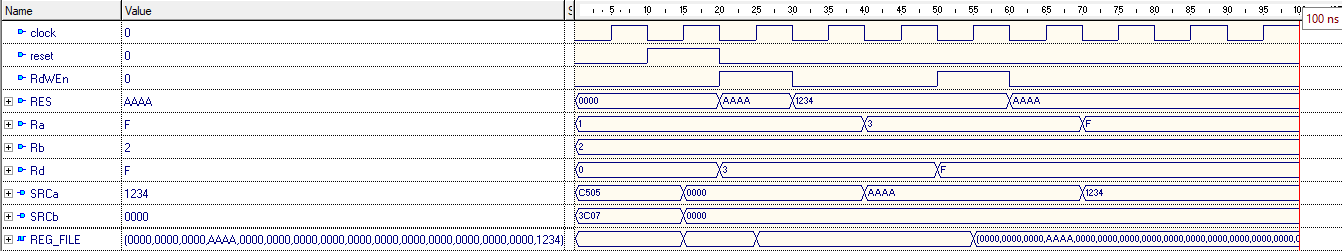
\includegraphics[width=1.1\textwidth, height=4cm]{Register simulation.png}
  \caption{Register File simulation waveform.}
  \label{fig:reg_sim}
\end{figure}



\subsection{Arithmetic Logic Unit (ALU)}

The ALU (\texttt{ALU.vhd}) is a \textbf{purely combinational} 16-bit processing unit
with no clock input. It evaluates its output immediately whenever any input changes.
The entity has three ports:

\begin{itemize}
  \item \texttt{ABUS[15:0]} — first operand (source register A).
  \item \texttt{BBUS[15:0]} — second operand (source register B).
  \item \texttt{CTRL[3:0]} — 4-bit opcode (only the lower 3 bits are used by the ALU;
        all ALU opcodes satisfy \texttt{CTRL[3] = '0'}).
  \item \texttt{ALU\_OUT[15:0]} — computed result.
\end{itemize}

A single \texttt{process} statement with sensitivity list \texttt{(ABUS, BBUS, CTRL)}
implements a \texttt{case} statement over \texttt{CTRL}. Table~\ref{tab:alu_ops}
summarises the eight supported operations.

\begin{table}[H]
\centering
\caption{ALU instruction set.}
\label{tab:alu_ops}
\small
\begin{tabularx}{\textwidth}{@{}c l l Y@{}}
\toprule
\textbf{CTRL} & \textbf{Mnemonic} & \textbf{Operation} & \textbf{Description} \\
\midrule
0000 & ADD & ABUS + BBUS $\rightarrow$ ALU\_OUT & Unsigned 16-bit addition (wraps modulo $2^{16}$) \\
0001 & SUB & ABUS $-$ BBUS $\rightarrow$ ALU\_OUT & Unsigned 16-bit subtraction \\
0010 & AND & ABUS \& BBUS $\rightarrow$ ALU\_OUT & Bitwise AND \\
0011 & OR  & ABUS $|$ BBUS $\rightarrow$ ALU\_OUT & Bitwise OR \\
0100 & XOR & ABUS $\oplus$ BBUS $\rightarrow$ ALU\_OUT & Bitwise XOR (key encryption primitive) \\
0101 & NOT & $\sim$ABUS $\rightarrow$ ALU\_OUT & Bitwise complement of ABUS; BBUS ignored \\
0110 & MOV & ABUS $\rightarrow$ ALU\_OUT & Pass-through copy; BBUS ignored \\
0111 & NOP & 0x0000 $\rightarrow$ ALU\_OUT & No operation; write disabled at top level \\
\bottomrule
\end{tabularx}
\normalsize
\end{table}

Arithmetic operations (ADD, SUB) use the \texttt{ieee.numeric\_std} library's
\texttt{unsigned} type for unsigned binary arithmetic before converting the result
back to \texttt{std\_logic\_vector}. This approach avoids explicit adder components
and lets the synthesis tool choose an efficient carry-chain structure.

% ----------------------------------------------------------------
% [INSERT CODE SNIPPET: Full ALU.vhd — entity declaration and
%  architecture with the case statement for all 8 opcodes]
% ----------------------------------------------------------------

\begin{lstlisting}[caption={ALU entity and architecture (ALU.vhd).}, xleftmargin=-1cm, xrightmargin=-1cm,
                   label={lst:alu}]
entity ALU is
    port (
        ABUS    : in  std_logic_vector(15 downto 0);  
        BBUS    : in  std_logic_vector(15 downto 0);  
        CTRL    : in  std_logic_vector(3  downto 0);  
        ALU_OUT : out std_logic_vector(15 downto 0)   
    );
end entity ALU;
 
architecture rtl of ALU is
begin
    process(ABUS, BBUS, CTRL)
    begin
        case CTRL is
            when "0000" => ALU_OUT <= std_logic_vector(unsigned(ABUS) + unsigned(BBUS));
            when "0001" => ALU_OUT <= std_logic_vector(unsigned(ABUS) - unsigned(BBUS));
            when "0010" => ALU_OUT <= ABUS and BBUS;
            when "0011" => ALU_OUT <= ABUS or BBUS;
            when "0100" => ALU_OUT <= ABUS xor BBUS;
            when "0101" => ALU_OUT <= not ABUS;
            when "0110" => ALU_OUT <= ABUS;
            when "0111" => ALU_OUT <= (others => '0');
            when others => ALU_OUT <= (others => '0');
        end case;
    end process;
end architecture rtl;
\end{lstlisting}


\subsubsection{ALU TestBench}

The ALU testbench (\texttt{alu\_tb.vhd}) applies a fixed pair of operands
(\texttt{ABUS = 0xC505}, \texttt{BBUS = 0x6808}) and cycles through all eight
opcodes (\texttt{CTRL = "0000"} to \texttt{"0111"}) at 10~ns intervals.
\begin{lstlisting}[language=VHDL, xleftmargin=-1cm, xrightmargin=-1cm,
                   caption={VHDL Implementation of the ALU TB File}, 
                   label={lst:ALUTB_file}]
entity ALU_tb is
end entity ALU_tb;

architecture sim of ALU_tb is
    signal ABUS    : std_logic_vector(15 downto 0);
    signal BBUS    : std_logic_vector(15 downto 0);
    signal CTRL    : std_logic_vector(3  downto 0);
    signal ALU_OUT : std_logic_vector(15 downto 0);

begin
    UUT : entity work.ALU
        port map (
            ABUS    => ABUS,
            BBUS    => BBUS,
            CTRL    => CTRL,
            ALU_OUT => ALU_OUT
        );

    process
    begin
       ABUS <= x"C505"; BBUS <= x"6808"; CTRL <= "0000"; wait for 10 ns;
       ABUS <= x"C505"; BBUS <= x"6808"; CTRL <= "0001"; wait for 10 ns;
       ABUS <= x"C505"; BBUS <= x"6808"; CTRL <= "0010"; wait for 10 ns;
       ABUS <= x"C505"; BBUS <= x"6808"; CTRL <= "0011"; wait for 10 ns;
       ABUS <= x"C505"; BBUS <= x"6808"; CTRL <= "0100"; wait for 10 ns;
       ABUS <= x"C505"; BBUS <= x"0000"; CTRL <= "0101"; wait for 10 ns;
       ABUS <= x"C505"; BBUS <= x"0000"; CTRL <= "0110"; wait for 10 ns;
       ABUS <= x"C505"; BBUS <= x"6808"; CTRL <= "0111"; wait for 10 ns;

        wait;
    end process;
end architecture sim;
\end{lstlisting}

\subsubsection{Results and Analysis}
Table~\ref{tab:alu_results} summarizes the expected versus observed results for each operation. The observed values perfectly match the expected hexadecimal outputs, confirming the correctness of the combinational logic.

\begin{table}[H]
\centering
\caption{ALU testbench — expected simulation results.}
\label{tab:alu_results}
\begin{tabular}{cllcc}
\toprule
\textbf{Time} & \textbf{CTRL} & \textbf{Op} &
\textbf{Expected ALU\_OUT} & \textbf{Observed} \\
\midrule
 0–10 ns  & 0000 & ADD & 0x2D0D & \checkmark \\
10–20 ns  & 0001 & SUB & 0x5CFD & \checkmark \\
20–30 ns  & 0010 & AND & 0x4000 & \checkmark \\
30–40 ns  & 0011 & OR  & 0xED0D & \checkmark \\
40–50 ns  & 0100 & XOR & 0xAD0D & \checkmark \\
50–60 ns  & 0101 & NOT (BBUS=0) & 0x3AFA & \checkmark \\
60–70 ns  & 0110 & MOV (BBUS=0) & 0xC505 & \checkmark \\
70–80 ns  & 0111 & NOP & 0x0000 & \checkmark \\
\bottomrule
\end{tabular}
\end{table}

The timing relationship and signal transitions are further illustrated in the simulation waveform (Figure~\ref{fig:alu_sim}). As expected for combinational logic, the \texttt{ALU\_OUT} bus updates immediately following every change in the \texttt{CTRL} signal.

\begin{figure}[H]
  \centering
   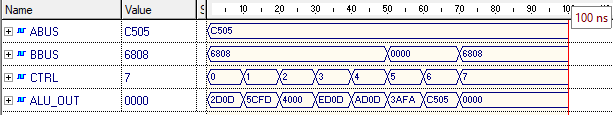
\includegraphics[width=1\textwidth, height=4cm]{ALU simulation.png}
  \caption{ALU simulation waveform — all eight operations.}
  \label{fig:alu_sim}
\end{figure}

\subsection{Shifter Unit}

The Shifter unit (\texttt{shifter.vhd}) is a purely combinational component
responsible for performing bitwise shift and rotation operations.
It receives a 16-bit input via \texttt{B\_Bus} (driven from BBUS) and a 4-bit
control signal \texttt{CTRL\_shifter}, and produces a 16-bit output
\texttt{shifter\_result}.

Only instructions with \texttt{CTRL[3] = '1'} are routed to the Shifter,
ensuring that it is activated exclusively for shift-related operations.
The supported operations are summarized in Table~\ref{tab:shifter_ops}.

\begin{table}[H]
\centering
\caption{Shifter instruction set.}
\label{tab:shifter_ops}
\small
\begin{tabularx}{\textwidth}{@{}c l l Y@{}}
\toprule
\textbf{CTRL} & \textbf{Mnemonic} & \textbf{VHDL Expression} & \textbf{Description} \\
\midrule
1000 & ROR8 & \texttt{B\_Bus(7:0) \& B\_Bus(15:8)} & Rotate right by 8 bits (byte swap) \\
1001 & ROR4 & \texttt{B\_Bus(3:0) \& B\_Bus(15:4)} & Rotate right by 4 bits (nibble rotation) \\
1010 & SLL8 & \texttt{B\_Bus(7:0) \& "00000000"}   & Logical left shift by 8 bits (zero fill) \\
\bottomrule
\end{tabularx}
\normalsize
\end{table}

A key distinction exists between rotation and logical shifting:
\begin{itemize}
  \item \textbf{Rotation (ROR8, ROR4):} Bits shifted out from one end of the word
        are reintroduced at the opposite end, preserving all information.
  \item \textbf{Logical Shift (SLL8):} Bits shifted out are discarded, and the
        vacated positions are filled with zeros, resulting in information loss.
\end{itemize}

To illustrate these operations, consider the input \texttt{0xBAA0}:
\begin{align*}
  \text{ROR8:} \quad & \texttt{0xBAA0} \rightarrow \texttt{0xA0BA} \\
  \text{ROR4:} \quad & \texttt{0xBAA0} \rightarrow \texttt{0x0BAA} \\
  \text{SLL8:} \quad & \texttt{0xBAA0} \rightarrow \texttt{0xA000}
\end{align*}

The following listing presents the VHDL implementation of the Shifter unit,
illustrating how the control signal selects the corresponding shift or rotation operation.
\begin{lstlisting}[language=VHDL, xleftmargin=-1cm, xrightmargin=-1cm,
caption={VHDL Implementation of the Shifter File},
label={lst:shifter_file}]
entity SHIFTER is
    port (	
        B_Bus          : in  std_logic_vector(15 downto 0);
        CTRL_shifter   : in  std_logic_vector(3 downto 0);
        shifter_result : out std_logic_vector(15 downto 0)
    );
end entity;

architecture behaviour of SHIFTER is
begin 
    process(B_Bus, CTRL_shifter)
    begin
        case CTRL_shifter is   
            when "1000" =>   -- Rotate Right 8-bit
			    shifter_result <= B_Bus(7 downto 0) & B_Bus(15 downto 8); 
			
            when "1001" =>   -- Rotate Right 4-bit
			    shifter_result <= B_Bus(3 downto 0) & B_Bus(15 downto 4); 
			
            when "1010" =>   -- Shift Left 8-bit
                shifter_result <= B_Bus(7 downto 0) & "00000000"; 
                        
            when others => 
                shifter_result <= (others => '0');
        end case;           
    end process;
end architecture;
\end{lstlisting}

\subsubsection{Shifter Simulation}

To verify functionality, a testbench applies a fixed input
\texttt{B\_Bus = 0x1234} while cycling through the control codes
\texttt{"1000"}, \texttt{"1001"}, \texttt{"1010"}, and \texttt{"0000"}
at 10~ns intervals.\\
The testbench used to validate the Shifter functionality is shown below.
It applies different control inputs over time and observes the resulting output behavior.

\begin{lstlisting}[language=VHDL, xleftmargin=-1cm, xrightmargin=-1cm,
caption={VHDL Implementation of the Shifter Testbench},
label={lst:shifter_tb_file}]
entity tb_shifter is
end entity;

architecture test of tb_shifter is
    signal B_Bus_tb          : std_logic_vector(15 downto 0) := (others => '0');
    signal CTRL_shifter_tb   : std_logic_vector(3 downto 0)  := (others => '0');
    signal shifter_result_tb : std_logic_vector(15 downto 0);
begin
    UUT: entity work.shifter
        port map (
            B_Bus => B_Bus_tb, CTRL_shifter => CTRL_shifter_tb,
            shifter_result => shifter_result_tb
        );
 
    test_proc: process
    begin 
        B_Bus_tb <= x"1234"; 
        
        CTRL_shifter_tb <= "1000";
        wait for 10 ns;
    
        CTRL_shifter_tb <= "1001";
        wait for 10 ns;
        
        CTRL_shifter_tb <= "1010";
        wait for 10 ns;
        
        CTRL_shifter_tb <= "0000";
        wait for 10 ns;

        wait;
    end process;
end architecture;
\end{lstlisting}

The expected outputs for each case are listed in
Table~\ref{tab:shifter_results}.

\begin{table}[H]
\centering
\caption{Shifter testbench — expected simulation results (input: 0x1234).}
\label{tab:shifter_results}
\small
\begin{tabularx}{\textwidth}{@{}c l l Y@{}}
\toprule
\textbf{CTRL} & \textbf{Op} & \textbf{Expected Output} & \textbf{Derivation} \\
\midrule
1000 & ROR8 & 0x3412 & Low byte (0x34) moves to high position; high byte (0x12) wraps to low \\
1001 & ROR4 & 0x4123 & Entire 16-bit word rotated right by 4 bits \\
1010 & SLL8 & 0x3400 & Low byte shifted left; lower bits zero-filled \\
0000 & N/A  & 0x0000 & Default (\texttt{others}) case: output cleared \\
\bottomrule
\end{tabularx}
\normalsize
\end{table}

The waveform in Figure~\ref{fig:shifter_sim} confirms the correct behavior
of the Shifter unit across all tested control signals. Each operation
produces the expected output at the corresponding time interval, matching
the results listed in Table~\ref{tab:shifter_results}.

\begin{figure}[H]
  \centering
  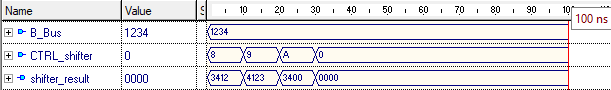
\includegraphics[width=\textwidth, height=4cm]{Shifter simulation.png}
    \caption{Shifter simulation waveform showing ROR8, ROR4, SLL8, and default.}
  \label{fig:shifter_sim}
\end{figure}

\subsection{Non-Linear Lookup Unit (LUT / S-Box)}

The LUT module (\texttt{LUT.vhd}) implements the \textbf{non-linear substitution}
function, which is a fundamental cryptographic primitive used to resist linear
and differential attacks. It operates on the lower byte of ABUS
(\texttt{ABUS[7:0]}), replacing it with a substituted value derived from two
4-bit S-Boxes (SBOX\_1 and SBOX\_2), while the upper byte
(\texttt{ABUS[15:8]}) passes through unchanged.

\subsubsection{Architecture}

The 8-bit input \texttt{LUT\_in} is divided into two 4-bit nibbles:
\begin{itemize}
  \item \texttt{LHS\_in = LUT\_in[7:4]} — processed by SBOX\_1.
  \item \texttt{RHS\_in = LUT\_in[3:0]} — processed by SBOX\_2.
\end{itemize}

Each S-Box is implemented using a 16-entry \texttt{with/select} statement,
mapping every possible 4-bit input to a unique 4-bit output. The results
(\texttt{LHS\_out} and \texttt{RHS\_out}) are concatenated to produce:
\[
\texttt{LUT\_out} = \texttt{LHS\_out} \;\|\; \texttt{RHS\_out}
\]

At the system level, the final 16-bit output is formed as:
\[
\texttt{LUT\_OUT} = \texttt{ABUS[15:8]} \;\|\; \texttt{LUT\_out}
\]

The complete substitution mappings are shown in
Table~\ref{tab:sbox1} and Table~\ref{tab:sbox2}.

% =========================
% SBOX TABLES (unchanged)
% =========================

\begin{table}[H]
\centering
\caption{S-Box 1 (SBOX\_1) — upper nibble substitution.}
\label{tab:sbox1}
\begin{tabular}{cc|cc|cc|cc}
\toprule
\textbf{In} & \textbf{Out} & \textbf{In} & \textbf{Out} &
\textbf{In} & \textbf{Out} & \textbf{In} & \textbf{Out} \\
\midrule
0x0 & 0x1 & 0x4 & 0xD & 0x8 & 0xE & 0xC & 0xA \\
0x1 & 0xB & 0x5 & 0x6 & 0x9 & 0x8 & 0xD & 0x2 \\
0x2 & 0x9 & 0x6 & 0xF & 0xA & 0x7 & 0xE & 0x5 \\
0x3 & 0xC & 0x7 & 0x3 & 0xB & 0x4 & 0xF & 0x0 \\
\bottomrule
\end{tabular}
\end{table}

\begin{table}[H]
\centering
\caption{S-Box 2 (SBOX\_2) — lower nibble substitution.}
\label{tab:sbox2}
\begin{tabular}{cc|cc|cc|cc}
\toprule
\textbf{In} & \textbf{Out} & \textbf{In} & \textbf{Out} &
\textbf{In} & \textbf{Out} & \textbf{In} & \textbf{Out} \\
\midrule
0x0 & 0xF & 0x4 & 0xB & 0x8 & 0x9 & 0xC & 0x3 \\
0x1 & 0x0 & 0x5 & 0xE & 0x9 & 0x2 & 0xD & 0x4 \\
0x2 & 0xD & 0x6 & 0x5 & 0xA & 0xC & 0xE & 0x8 \\
0x3 & 0x7 & 0x7 & 0xA & 0xB & 0x1 & 0xF & 0x6 \\
\bottomrule
\end{tabular}
\end{table}

\subsubsection{Worked Example}

Consider \texttt{ABUS = 0xAB5C} with opcode \texttt{CTRL = "1011"}:

\begin{enumerate}
  \item Upper byte (\texttt{0xAB}) remains unchanged.
  \item Lower byte (\texttt{0x5C}) is split into \texttt{0x5} and \texttt{0xC}.
  \item \texttt{SBOX\_1[0x5] = 0x6}, \texttt{SBOX\_2[0xC] = 0x3}.
  \item \texttt{LUT\_out = 0x63}.
  \item Final output: \texttt{0xAB63}.
\end{enumerate}

% =========================
% LUT CODE
% =========================
The following listing shows the VHDL implementation of the LUT unit,
including the S-Box mappings and output construction logic.

\begin{lstlisting}[language=VHDL, xleftmargin=-1cm, xrightmargin=-1cm,
caption={VHDL Implementation of the LUT (S-Box) File},
label={lst:lut_file}]
entity LUT is
	port(
		LUT_in : in	std_logic_vector(7 downto 0);
		LUT_out : out std_logic_vector(7 downto 0)
	);
end entity;

architecture rtl of LUT is
signal LHS_in, LHS_out, RHS_in, RHS_out : std_logic_vector(3 downto 0);
begin
	LHS_in <= LUT_in(7 downto 4);
	RHS_in <= LUT_in(3 downto 0);
	
	SBOX_1 : block is
	begin
		with LHS_in select
			LHS_out <= "0001" when "0000",
			           "1011" when "0001",
					   "1001" when "0010",
					   "1100" when "0011",
					   "1101" when "0100",
					   "0110" when "0101",
					   "1111" when "0110",
					   "0011" when "0111",
					   "1110" when "1000",
					   "1000" when "1001",
					   "0111" when "1010",
					   "0100" when "1011",
					   "1010" when "1100",
					   "0010" when "1101",
					   "0101" when "1110",
					   "0000" when "1111",
					   "XXXX" when others;
	end block;
	
	SBOX_2 : block is
	begin
		with RHS_in select
			RHS_out <= "1111" when "0000",
			           "0000" when "0001",
					   "1101" when "0010",
					   "0111" when "0011",
					   "1011" when "0100",
					   "1110" when "0101",
					   "0101" when "0110",
					   "1010" when "0111",
					   "1001" when "1000",
					   "0010" when "1001",
					   "1100" when "1010",
					   "0001" when "1011",
					   "0011" when "1100",
					   "0100" when "1101",
					   "1000" when "1110",
					   "0110" when "1111",
					   "XXXX" when others;
	end block;
	
	LUT_out <= LHS_out & RHS_out;
end architecture;

\end{lstlisting}

\subsubsection{LUT Simulation}

To verify correctness, a testbench applies all possible 8-bit inputs
(\texttt{0x00–0xFF}) to \texttt{LUT\_in} at fixed time intervals.
For each input, the output is compared against the expected value
derived from SBOX\_1 and SBOX\_2.

% =========================
% LUT TB CODE
% =========================
The testbench implementation used for verification is shown below.
It systematically iterates through all input combinations.

\begin{lstlisting}[language=VHDL, xleftmargin=-1cm, xrightmargin=-1cm,
caption={VHDL Implementation of the LUT Testbench},
label={lst:lut_tb_file}]
entity LUT_tb is
end entity;

architecture sim of LUT_tb is
signal LUT_in, LUT_out : std_logic_vector(7 downto 0);
begin
	DUT : entity work.LUT
		port map(
			LUT_in => LUT_in, LUT_out => LUT_out
		); 
		
	process is
	begin
		for i in 0 to 255 loop
			LUT_in <= std_logic_vector(to_unsigned(i, 8));
			wait for 50 ns;
		end loop;
		wait;
	end process;
end architecture;
\end{lstlisting}

Selected verification results are summarized in
Table~\ref{tab:lut_results}.

\begin{table}[H]
\centering
\caption{LUT testbench — selected verification results.}
\label{tab:lut_results}
\begin{tabular}{ccccc}
\toprule
\textbf{LUT\_in} & \textbf{Upper nibble} & \textbf{SBOX\_1} &
\textbf{Lower nibble} & \textbf{SBOX\_2} \\
\midrule
0x5C & 5 & 6 & C & 3 → \textbf{0x63} \\
0x00 & 0 & 1 & 0 & F → \textbf{0x1F} \\
0xFF & F & 0 & F & 6 → \textbf{0x06} \\
0xAB & A & 7 & B & 1 → \textbf{0x71} \\
\bottomrule
\end{tabular}
\end{table}

The waveform in Figure~\ref{fig:lut_sim} confirms the correct operation
of the LUT across different inputs, matching the expected substitution behavior.

\begin{figure}[H]
  \centering
  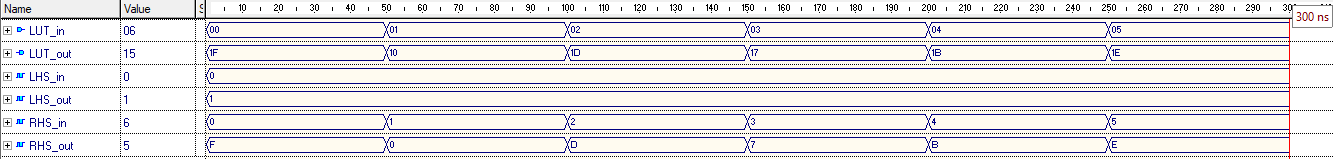
\includegraphics[width=1.1\textwidth, height=4cm]{LUT simulation.png}
  \caption{LUT (S-Box) simulation waveform.}
  \label{fig:lut_sim}
\end{figure}

\newpage
\section{Design Details}

\subsection{Component Interaction and Data Flow}

Figure~\ref{fig:dataflow} illustrates how the five major components interact
to process a single instruction from input to write-back.

\begin{figure}[H]
\centering
\begin{tikzpicture}[scale=0.75, transform shape,
    >=Stealth,
    blk/.style={
        draw=black!40, rounded corners=5pt,
        minimum width=3cm, minimum height=1.2cm,
        align=center, text=white,
        font=\sffamily\footnotesize\bfseries,
        fill=#1
    },
    lbl/.style={
        font=\sffamily\scriptsize,
        fill=white,
        inner sep=2pt,
        rounded corners=2pt
    }
]

% =========================
% TOP: INPUT
% =========================
\node[blk=clkcolor] (IN)
{External Inputs\\ 
        \texttt{CTRL[3:0]}\\[2pt]
       \texttt{Ra[3:0]}\\[2pt]
       \texttt{Rb[3:0]}\\[2pt]
       \texttt{Rd[3:0]}\\[2pt]
       \texttt{clock}\\[2pt]
       \texttt{reset}};

% =========================
% PIPELINE
% =========================
\node[blk=pipecolor, below=1.8cm of IN] (PIPE)
 {Input Pipeline\\Register\\[2pt]
       \texttt{\tiny Process\_control}};

\draw[->, thick] (IN) -- (PIPE)
node[midway, right, lbl]{CTRL, Ra, Rb, Rd};

% =========================
% REGISTER FILE
% =========================
\node[blk=regcolor, below=2cm of PIPE] (REG)
 {Register File\\$16 \times 16$-bit\\[2pt]
       \texttt{\tiny R0 -- R15}};

\draw[->, thick] (PIPE) -- (REG)
node[midway, right, lbl]{addr/control};

% =========================
% FUNCTION UNITS (SIDE BY SIDE)
% =========================
\node[blk=alucolor, below=2cm of REG, xshift=-5cm] (ALU)
 {ALU\\[2pt]
       \texttt{\tiny ADD/SUB/AND}\\
       \texttt{\tiny OR/XOR/NOT}\\
       \texttt{\tiny MOV/NOP}};

\node[blk=shiftcolor, right=2.5cm of ALU] (SHF)
 {Shifter\\[2pt]
       \texttt{\tiny ROR8 / ROR4 / SLL8}};

\node[blk=lutcolor, right=2.5cm of SHF] (LUT)
  {LUT / S-Box\\[2pt]
       \texttt{\tiny SBOX\_1 (hi nibble)}\\
       \texttt{\tiny SBOX\_2 (lo nibble)}};

% =========================
% ABUS (clean split)
% =========================
\draw[->, thick, color=regcolor]
(REG.south) -- ++(0,-0.8) -| (ALU.north)
node[pos=0.25, left, lbl]{ABUS};

\draw[->, thick, color=regcolor]
(REG.south) -- ++(0,-0.8) -| (LUT.north)
node[pos=0.75, right, lbl]{ABUS[7:0]};

% =========================
% BBUS (FIXED PROPERLY)
% =========================
\draw[->, thick, color=regcolor]
(REG.east) -- ++(1,0) |- (SHF.north)
node[pos=0.4, right, lbl]{BBUS};

\draw[->, thick, color=regcolor!70]
(REG.east) -- ++(1,0) |- (ALU.north)
node[pos=0.7, right, lbl]{BBUS};

% =========================
% MUX
% =========================
\node[blk=muxcolor, below=3cm of SHF] (MUX)
 {Control\\MUX\\[6pt]
       \texttt{\tiny CTRL[3]=0}\\
       \texttt{\tiny $\rightarrow$ ALU}\\[3pt]
       \texttt{\tiny "1011"}\\
       \texttt{\tiny $\rightarrow$ LUT}\\[3pt]
       \texttt{\tiny else}\\
       \texttt{\tiny $\rightarrow$ Shifter}};

% outputs to mux
\draw[->, thick] (ALU.south) |- (MUX.west)
node[pos=0.3, lbl]{ALU};

\draw[->, thick] (SHF.south) -- (MUX)
node[midway, right, lbl]{SHIFT};

\draw[->, thick] (LUT.south) |- (MUX.east)
node[pos=0.3, lbl]{LUT};

% =========================
% RESULT
% =========================
\node[blk=clkcolor, below=2cm of MUX] (RES)
 {RESULT\\[2pt]\texttt{\tiny 16-bit bus}};

\draw[->, very thick] (MUX) -- (RES)
node[midway, right, lbl]{RES};

% =========================
% WRITE BACK (clean bottom loop)
% =========================
\draw[->, very thick, color=clkcolor]
(RES.south) -- ++(0,-1.5) -- ++(-6,0) |- (REG.west)
node[midway, below, lbl]{Write-back to Rd};

% =========================
% CONTROL (clean, no overlap)
% =========================
\draw[->, dashed]
(PIPE.east) -- ++(2,0) |- (MUX.north)
node[pos=0.7, lbl]{MUX sel};

\end{tikzpicture}
\caption{Detailed data-flow diagram of CryptoCore-16.}
\label{fig:dataflow}
\end{figure}



The interaction between components follows the sequence below for a representative
instruction \texttt{XOR R1, R8 $\rightarrow$ R7}:

\begin{enumerate}
  \item \textbf{Clock cycle N — input capture:}
        On the rising edge, the \texttt{Process\_control} process latches
        \texttt{CTRL = "0100"}, \texttt{Ra = "0001"}, \texttt{Rb = "1000"},
        \texttt{Rd = "0111"} from the primary inputs.
        \texttt{ctrl\_tmp $\leftarrow$ "0100"}, \texttt{RdWEn $\leftarrow$ '1'}.

  \item \textbf{Combinational phase (same cycle):}
        The register file immediately drives
        \texttt{ABUS = REG[1] = 0xC505} and \texttt{BBUS = REG[8] = 0x6808}.
        The ALU, Shifter, and LUT all evaluate concurrently:
        \begin{itemize}
          \item ALU: \texttt{0xC505 XOR 0x6808 = 0xAD0D} $\rightarrow$ \texttt{ALU\_OUT}.
          \item Shifter: result irrelevant (CTRL[3] = 0, will not be selected).
          \item LUT: result irrelevant (CTRL $\neq$ \texttt{"1011"}).
        \end{itemize}
        Control MUX: since \texttt{ctrl\_tmp[3] = '0'}, \texttt{RES $\leftarrow$ ALU\_OUT = 0xAD0D}.

  \item \textbf{Clock cycle N+1 — write-back:}
        On the next rising edge, since \texttt{RdWEn = '1'},
        \texttt{REG[7] $\leftarrow$ 0xAD0D}.
\end{enumerate}

\subsection{Control Signals and Opcode Usage}

The 4-bit \texttt{CTRL} opcode is the sole selector for all routing and write-back
decisions. Table~\ref{tab:full_isa} presents the complete instruction set architecture.

\begin{table}[H]
\centering
\caption{Complete Instruction Set Architecture (ISA) of CryptoCore-16.}
\label{tab:full_isa}
\small
\begin{tabularx}{\textwidth}{@{}c l l Y l@{}}
\toprule
\textbf{CTRL} & \textbf{Mnemonic} & \textbf{Unit} & \textbf{Operation} & \textbf{Write?} \\
\midrule
0000 & ADD  & ALU     & ABUS + BBUS $\rightarrow$ Rd   & Yes \\
0001 & SUB  & ALU     & ABUS $-$ BBUS $\rightarrow$ Rd & Yes \\
0010 & AND  & ALU     & ABUS \& BBUS $\rightarrow$ Rd  & Yes \\
0011 & OR   & ALU     & ABUS $|$ BBUS $\rightarrow$ Rd & Yes \\
0100 & XOR  & ALU     & ABUS $\oplus$ BBUS $\rightarrow$ Rd & Yes \\
0101 & NOT  & ALU     & $\sim$ABUS $\rightarrow$ Rd    & Yes \\
0110 & MOV  & ALU     & ABUS $\rightarrow$ Rd          & Yes \\
0111 & NOP  & ALU     & No operation                   & \textbf{No} \\
1000 & ROR8 & Shifter & Rotate BBUS right 8 $\rightarrow$ Rd & Yes \\
1001 & ROR4 & Shifter & Rotate BBUS right 4 $\rightarrow$ Rd & Yes \\
1010 & SLL8 & Shifter & Shift BBUS left 8 $\rightarrow$ Rd  & Yes \\
1011 & LUT  & LUT     & S-Box(ABUS[7:0]) $\rightarrow$ Rd  & Yes \\
\bottomrule
\end{tabularx}
\normalsize
\end{table}

The control MUX logic inside \texttt{structural\_combinational\_logic\_block.vhd}
uses a two-level decision:
\begin{enumerate}
  \item If \texttt{CTRL[3] = '0'} $\Rightarrow$ select ALU output (instructions 0000–0111).
  \item Else if \texttt{CTRL = "1011"} $\Rightarrow$ select LUT output.
  \item Else $\Rightarrow$ select Shifter output (instructions 1000, 1001, 1010).
\end{enumerate}

\subsection{Instruction Format}

Every instruction is encoded in a 16-bit word with four 4-bit fields:

\begin{center}
\begin{tabular}{|c|c|c|c|}
\hline
\texttt{CTRL[3:0]} & \texttt{Ra[3:0]} & \texttt{Rb[3:0]} & \texttt{Rd[3:0]} \\
\hline
Opcode & Source A & Source B & Destination \\
\hline
\end{tabular}
\end{center}

\section{VHDL Code Description}

\subsection{Overall Code Structure}

The project is organised into six VHDL source files and six corresponding testbench files,
listed in Table~\ref{tab:files}.

\begin{table}[H]
\centering
\caption{Project file structure.}
\label{tab:files}
\small
\begin{tabularx}{\textwidth}{@{}l Y@{}}
\toprule
\textbf{Source file} & \textbf{Description} \\
\midrule
\texttt{ALU.vhd}                            & Arithmetic Logic Unit (combinational) \\
\texttt{shifter.vhd}                        & Shifter / Rotator (combinational) \\
\texttt{LUT.vhd}                            & S-Box non-linear lookup (combinational) \\
\texttt{register.vhd}                       & 16$\times$16 Register File (synchronous write) \\
\texttt{combinational\_logic\_block.vhd}    & Structural integration of ALU, Shifter, LUT + MUX \\
\texttt{crypto\_core16.vhd}                 & Top-level entity — full coprocessor \\
\midrule
\textbf{Testbench file} & \textbf{Entity under test} \\
\midrule
\texttt{ALU\_tb.vhd}                        & \texttt{ALU} \\
\texttt{shifter\_tb.vhd}                    & \texttt{SHIFTER} \\
\texttt{LUT\_tb.vhd}                        & \texttt{LUT} \\
\texttt{register\_tb.vhd}                   & \texttt{register\_file} \\
\texttt{combinational\_logic\_block\_tb.vhd}& \texttt{structural\_combinational\_logic\_block} \\
\texttt{crypto\_core16\_tb.vhd}             & \texttt{crypto\_core16} \\
\bottomrule
\end{tabularx}
\normalsize
\end{table}

\subsection{Full Signal Flow: From Input to Output}

The following narrative traces the complete journey of an instruction through
every layer of the hierarchy:

\begin{enumerate}[leftmargin=*, label=\textbf{Step \arabic*:}]

  \item \textbf{External Input.}
        The host system asserts \texttt{CTRL[3:0]}, \texttt{Ra[3:0]}, \texttt{Rb[3:0]},
        and \texttt{Rd[3:0]} on the primary input pins of \texttt{crypto\_core16}.

  \item \textbf{Pipeline Register Capture.}
        On the rising edge of \texttt{clock}, the top-level
        \texttt{Process\_control} logic samples \texttt{CTRL} into
        \texttt{ctrl\_tmp} and sets \texttt{RdWEn} according to whether the opcode is NOP.

  \item \textbf{Register File Read.}
        Combinatorially (zero latency), the register file decodes \texttt{Ra} and
        \texttt{Rb} as integer indices and drives the corresponding stored 16-bit
        values onto \texttt{ABUS} (\texttt{SRCa}) and \texttt{BBUS} (\texttt{SRCb}).

  \item \textbf{Parallel Execution.}
        The combinational logic block receives \texttt{ABUS}, \texttt{BBUS}, and
        \texttt{ctrl\_tmp}. All three units compute simultaneously:
        \begin{itemize}
          \item \textbf{ALU} evaluates all eight operations and asserts \texttt{ALU\_OUT}.
          \item \textbf{Shifter} evaluates all three shift/rotate options and asserts
                \texttt{SHIFT\_OUT}.
          \item \textbf{LUT} performs nibble substitution on \texttt{ABUS[7:0]} and
                concatenates the upper byte to form \texttt{LUT\_OUT}.
        \end{itemize}

  \item \textbf{MUX Selection.}
        The \texttt{CONTROL\_MUX} process evaluates \texttt{ctrl\_tmp[3]} (and
        \texttt{ctrl\_tmp} in full for the LUT case) and routes exactly one of
        \texttt{ALU\_OUT}, \texttt{SHIFT\_OUT}, or \texttt{LUT\_OUT} to
        the output \texttt{RES}.

  \item \textbf{Write-Back.}
        \texttt{RES} feeds back into the register file's \texttt{RES} port.
        On the next rising edge of \texttt{clock}, if \texttt{RdWEn = '1'},
        the value is written into register \texttt{Rd}, completing the instruction cycle.

\end{enumerate}

% ============================================================
\chapter{Inputs and Outputs}
% ============================================================

\section{Primary Interface Signals}

Table~\ref{tab:io} lists all signals at the top-level boundary of \texttt{crypto\_core16}.

\begin{table}[H]
\centering
\caption{Top-level input and output signals of CryptoCore-16.}
\label{tab:io}
\small
\begin{tabularx}{\textwidth}{@{}p{1cm} c c Y@{}}
\toprule
\textbf{Signal} & \textbf{Dir.} & \textbf{Width} & \textbf{Description} \\
\midrule
\texttt{clock}  & IN  & 1 bit  & System clock. All synchronous operations
                                  (register write, input pipeline) trigger on
                                  the rising edge. \\
\texttt{reset}  & IN  & 1 bit  & Active-high synchronous reset. Clears all
                                  registers to 0x0000 and forces NOP. \\
\texttt{CTRL}   & IN  & 4 bits & Instruction opcode. Encodes which of the 12
                                  operations to perform and which unit to use. \\
\texttt{Ra}     & IN  & 4 bits & Address of source register A. Selects one of
                                  16 registers to drive ABUS. \\
\texttt{Rb}     & IN  & 4 bits & Address of source register B. Selects one of
                                  16 registers to drive BBUS. \\
\texttt{Rd}     & IN  & 4 bits & Address of the destination register. The
                                  computation result is written here on the
                                  next clock edge (unless NOP). \\
\bottomrule
\end{tabularx}
\normalsize
\end{table}

\textbf{Note:} The top-level entity has \emph{no output ports}. The result bus
\texttt{RESULT} is an internal signal that loops from the combinational logic block
back into the register file write port. This is a deliberate design choice: the
coprocessor stores all computed results in its internal register file; the host CPU
retrieves them by reading the register file through a separate bus-interface
(not included in this baseline implementation).

\section{Internal Signal Summary}

\begin{table}[H]
\centering
\caption{Key internal signals and their roles.}
\label{tab:internal_signals}
\small
\begin{tabularx}{\textwidth}{@{}p{1.5cm} p{1.5cm} X@{}}\toprule
\textbf{Signal} & \textbf{Width} & \textbf{Description} \\
\midrule
\texttt{ctrl\_tmp}  & 4 bits  & Registered copy of \texttt{CTRL}.
                                  Ensures stable opcode during computation. \\
\texttt{RdWEn}      & 1 bit   & Write-enable for the register file.
                                  Cleared for NOP; set for all other opcodes. \\
\texttt{ABUS}       & 16 bits & Data bus carrying the value of register Ra
                                  to the combinational logic block. \\
\texttt{BBUS}       & 16 bits & Data bus carrying the value of register Rb
                                  to the combinational logic block. \\
\texttt{RESULT}     & 16 bits & Output of the control MUX. Carries the computed
                                  result back to the register file write port. \\
\texttt{ALU\_OUT}   & 16 bits & Output of the ALU unit (internal to comb. block). \\
\texttt{SHIFT\_OUT} & 16 bits & Output of the Shifter unit. \\
\texttt{LUT\_OUT}   & 16 bits & Output of the LUT unit (upper byte pass-through
                                  + substituted lower byte). \\
\bottomrule
\end{tabularx}
\normalsize
\end{table}

% ============================================================
\chapter{Schematic Diagram}
% ============================================================
  \vspace{-0.5cm}

\section{Active-HDL™ Functional Schematic}

Prior to hardware synthesis, a functional schematic of the CryptoCore-16 was manually constructed within the Aldec Active-HDL™ as illustrated in Figure \ref{fig:active_hdl_schem}. This process allowed for a custom visualization of the RTL architecture, ensuring a clear mapping of the VHDL entities before simulation.

\begin{figure}[H]
    \centering
    \makebox[\textwidth][c]{%
         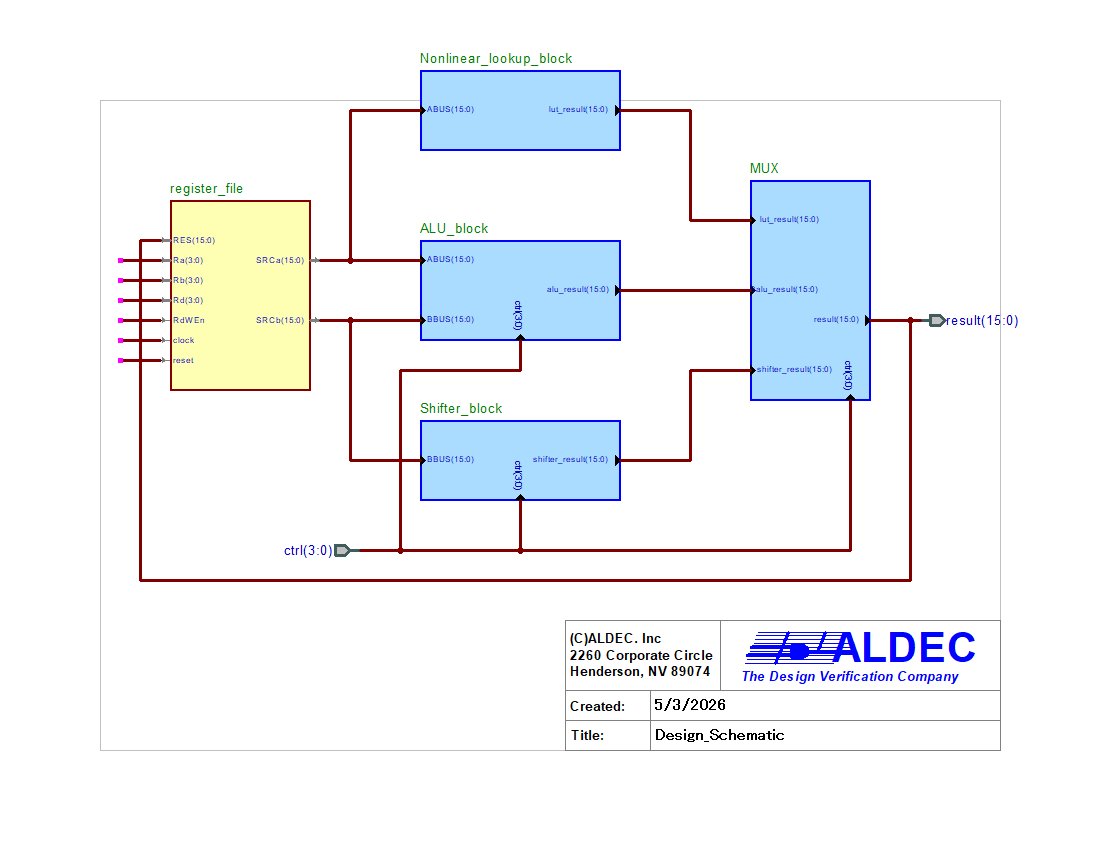
\includegraphics[width=1.1\textwidth]{Design_Schematic.png}%
    }
  \caption{Functional RTL schematic generated in Active-HDL.}
  \label{fig:active_hdl_schem}
  
\end{figure}

\newpage

\section{Quartus® Prime Schematic Overview}

The complete schematic of CryptoCore-16 was generated by Quartus® Prime Lite Edition from the
synthesised VHDL source. The schematic reveals the structural hierarchy of the design
and the interconnection of all sub-components.


\begin{figure}[H]
    \centering
    \makebox[\textwidth][c]{%
         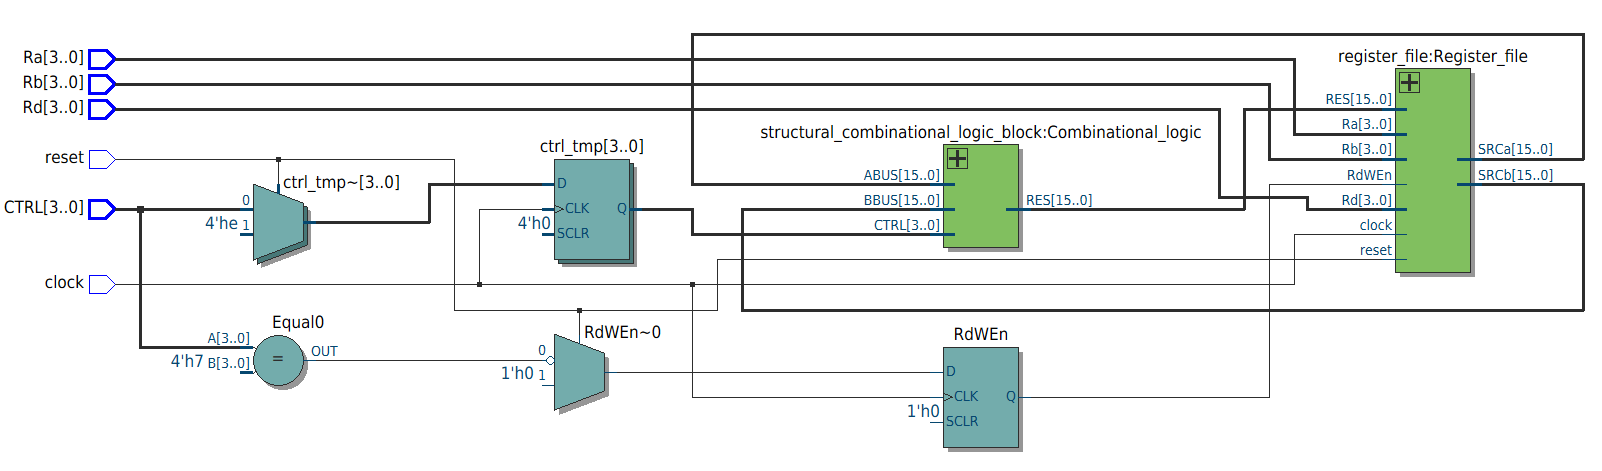
\includegraphics[width=1.1\textwidth]{top view schematic.png}%
    }
     \caption{Top-level schematic of CryptoCore-16.}
  \label{fig:top_schem}
\end{figure}



\section{Combinational Logic Block Schematic}


\begin{figure}[H]
    \centering
    \makebox[\textwidth][c]{%
        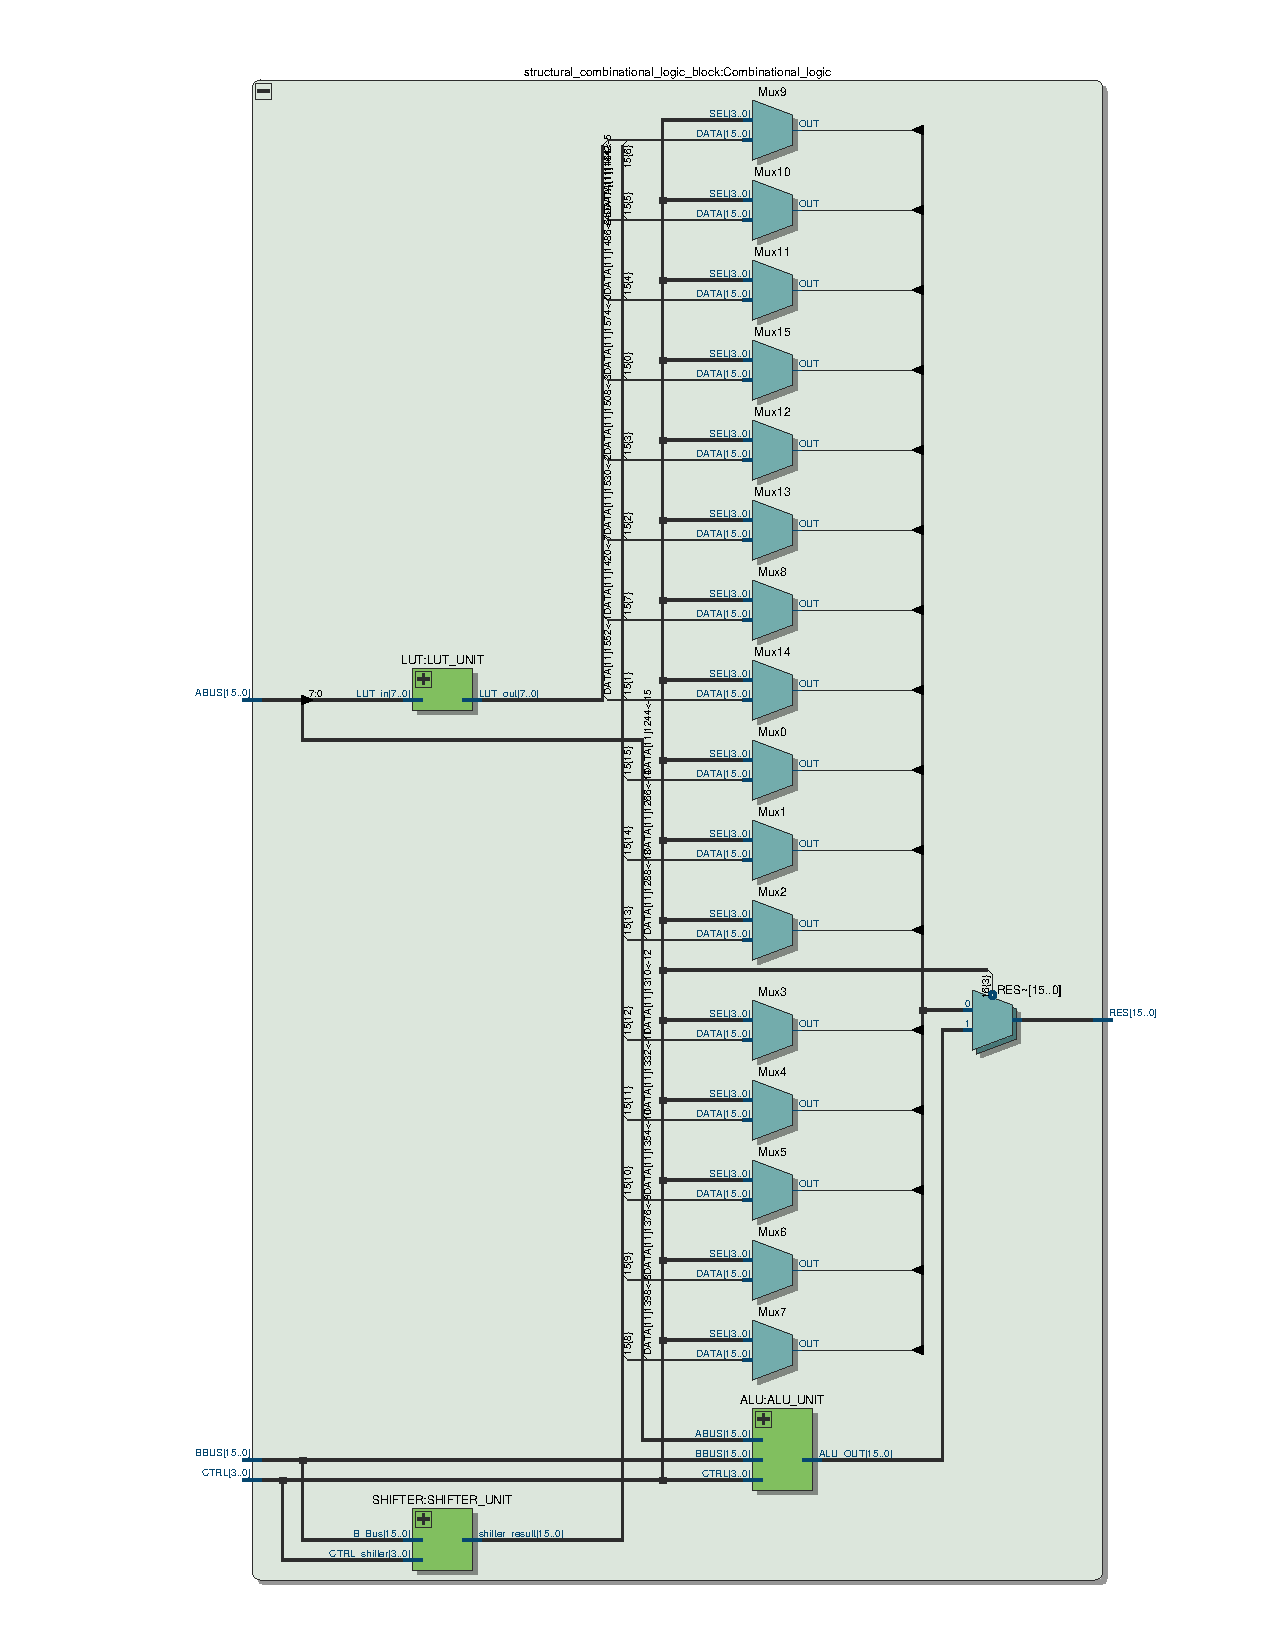
\includegraphics[width=1.2\textwidth]{compinational logic block schematic.pdf}%
    }
    \caption{Schematic diagram of the Combinational Logic Block.}
    \label{fig:comb_logic_schematic}
\end{figure}



% ============================================================
\chapter{Final Simulation Results}
% ============================================================

\section{Simulation Environment}

All simulations were performed using \textbf{Aldec Active-HDL} with a functional
(behavioural) simulation model. Each component was simulated independently before
the full system integration test was carried out. The simulation procedure for each
module was:

\begin{enumerate}
  \item Open the source file and its corresponding testbench in Active-HDL.
  \item Compile both files: \texttt{acom <source>.vhd} then \texttt{acom <tb>.vhd}.
  \item Launch simulation: \texttt{asim <tb\_entity> sim}.
  \item Add relevant signals to the waveform viewer.
  \item Execute: \texttt{run} (testbench ends automatically with \texttt{wait;}).
  \item Verify output values against expected results.
\end{enumerate}


\section{Combinational Logic Block Simulation}

The \texttt{Combinational\_logic\_block\_tb.vhd} exercises all three
data paths through the MUX by applying sequences of operands with different
\texttt{CTRL} values. Table~\ref{tab:comb_results} summarises the eight test cases written in \texttt{Combinational\_logic\_block\_tb.vhd}.


\subsection{Combinational logic block TB implementation}
\begin{lstlisting}[language=VHDL, xleftmargin=-1cm, xrightmargin=-1cm,
caption={VHDL Implementation of the CLB TB File},
label={lst:CLB_tb_file}]
entity structural_combinational_logic_block_tb is
end entity;

architecture sim of structural_combinational_logic_block_tb is
signal ABUS : std_logic_vector(15 downto 0);
signal BBUS : std_logic_vector(15 downto 0);
signal CTRL : std_logic_vector(3 downto 0);
signal RES  : std_logic_vector(15 downto 0);

begin
DUT: entity work.structural_combinational_logic_block
port map(
ABUS => ABUS,
BBUS => BBUS,
CTRL => CTRL,
RES  => RES
);

process	is
begin
	
-- Test 1: ALU path  (CTRL(3) = 0)
ABUS <= x"0005";
BBUS <= x"0003";
CTRL <= "0000";  -- ALU_SUM
wait for 10 ns;

-- Test 2: LUT path   (CTRL(3)=1 and CTRL(1:0)="11")
ABUS <= x"00AA";
BBUS <= x"0000";
CTRL <= "1011";  -- LUT
wait for 10 ns;

-- Test 3: SHIFTER path  (CTRL(3)=1 and not LUT)
ABUS <= x"0000";
BBUS <= x"000F";
CTRL <= "1000";  -- ROR8
wait for 10 ns;

-- Test 4: Another ALU case
ABUS <= x"0010";
BBUS <= x"0004";
CTRL <= "0001";	-- ALU_SUB
wait for 10 ns;

-- Test 5: Another shifter case
ABUS <= x"1234";
BBUS <= x"12FF";
CTRL <= "1010"; -- SLL8
wait for 10 ns;

-- Test 6: Another ALU case
ABUS <= x"1234";
BBUS <= x"12FF";
CTRL <= "0111"; -- NOP
wait for 10 ns;	 

-- Test 7: Another ALU case
ABUS <= x"1234";
BBUS <= x"12FF";
CTRL <= "0100"; -- XOR
wait for 10 ns;	 

-- Test 8: Another shifter case
ABUS <= x"1234";
BBUS <= x"12FF";
CTRL <= "1001"; -- ROR4
wait for 10 ns;	  

wait;

end process;
end architecture;

\end{lstlisting}

\begin{table}[H]
\centering
\caption{Combinational Logic Block testbench — expected results.}
\label{tab:comb_results}
\small
\begin{tabularx}{\textwidth}{@{}c c l Y l@{}}
\toprule
\textbf{Test} & \textbf{CTRL} & \textbf{Path} & \textbf{Inputs} & \textbf{Expected RES} \\
\midrule
1 & 0000 & ALU (ADD)  & ABUS=0x0005, BBUS=0x0003 & 0x0008 \\
2 & 1011 & LUT        & ABUS=0x00AA              & 0x00\textit{xx} (SBOX of 0xAA) \\
3 & 1000 & Shifter (ROR8) & BBUS=0x000F         & 0x0F00 \\
4 & 0001 & ALU (SUB)  & ABUS=0x0010, BBUS=0x0004 & 0x000C \\
5 & 1010 & Shifter (SLL8) & BBUS=0x12FF         & 0xFF00 \\
6 & 0111 & ALU (NOP)  & ABUS=0x1234, BBUS=0x12FF & 0x0000 \\
7 & 0100 & ALU (XOR)  & ABUS=0x1234, BBUS=0x12FF & 0x00CB \\
8 & 1001 & Shifter (ROR4) & BBUS=0x12FF         & 0xF12F \\
\bottomrule
\end{tabularx}
\normalsize
\end{table}

 
\begin{figure}[H]
  \centering
   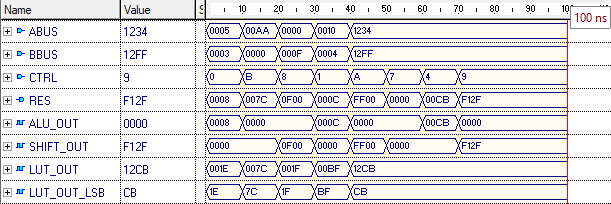
\includegraphics[width=1.1\textwidth]{Combinational Logic Block Simulation.png}
  \caption{Combinational Logic Block simulation waveform (Active-HDL capture).}
  \label{fig:comb_wave}
\end{figure}



% ============================================================
\section{Top-Level System Simulation}
% ============================================================

\subsection{Top-Level Source Code: \texttt{crypto\_core16.vhd}}

The top-level entity \texttt{crypto\_core16} is the structural integration
point of the entire coprocessor. Its port list is deliberately minimal — six
signals in total — because all data movement is handled internally through
the register file and the combinational logic block. The entity declares three
internal signals (\texttt{ABUS}, \texttt{BBUS}, \texttt{RESULT}) that serve
as the 16-bit data highways between the register file and the combinational
logic block, plus \texttt{ctrl\_tmp} (the registered opcode) and \texttt{RdWEn}
(write-enable). Two component instances are bound structurally: \texttt{register\_file}
and \texttt{structural\_combinational\_logic\_block}. A single clocked process,
\texttt{Process\_control}, provides the one-stage input pipeline.

\begin{lstlisting}[
  caption={Top-level coprocessor entity and architecture (crypto\_core16.vhd).},
  label={lst:core16}]
entity crypto_core16 is
	port(
		clock, reset : in std_logic;
	    CTRL, Ra, Rb, Rd : in std_logic_vector(3 downto 0)
	);
end entity;

architecture struct of crypto_core16 is
signal RdWEn : std_logic;
signal ctrl_tmp: std_logic_vector(3 downto 0);
signal ABUS, BBUS, RESULT : std_logic_vector(15 downto 0);
begin
	Register_file : entity work.register_file
		port map(
			clock => clock,
			reset => reset,
			RdWEn => RdWEn,
			RES => RESULT,
			Ra => Ra,
			Rb => Rb,
			Rd => Rd,
			SRCa => ABUS,
			SRCb => BBUS
		);
		
	Combinational_logic : entity work.structural_combinational_logic_block
		port map(
			ABUS => ABUS,
			BBUS => BBUS,
			CTRL => ctrl_tmp,
			RES => RESULT
		);
		
Process_control : process(clock)
begin
    if rising_edge(clock) then
        if reset = '1' then
            ctrl_tmp <= "0111";   -- NOP
            RdWEn    <= '0';      -- disable write
        else
            ctrl_tmp <= CTRL;

            if CTRL = "0111" then
                RdWEn <= '0';
            else
                RdWEn <= '1';
            end if;
        end if;
    end if;
end process;
end architecture;
\end{lstlisting}

\newpage
\paragraph{Key design decisions visible in the code.}
\begin{itemize}
  \item The \texttt{Combinational\_logic} instance receives \texttt{ctrl\_tmp},
        not the raw \texttt{CTRL} input. This one-cycle pipeline register ensures
        that the opcode presented to the ALU, Shifter, and LUT is stable and
        glitch-free throughout the entire combinational evaluation phase.
  \item \texttt{RESULT} is both the output of the combinational block and the
        write-data input of the register file. The single signal forms a closed
        feedback loop; the write is gated by \texttt{RdWEn} so it only commits
        on the next rising edge when the instruction is not a NOP.
  \item The top-level entity exposes \emph{no} output ports. All computed
        results reside inside the register file, consistent with the
        coprocessor design model where the host CPU retrieves values
        through a separate interface.
\end{itemize}

% ──────────────────────────────────────────────────────────
\subsection{Testbench Code: \texttt{crypto\_core16\_tb.vhd}}
% ──────────────────────────────────────────────────────────

The testbench \texttt{tb\_crypto} is structured into two concurrent processes:
a free-running \textbf{clock generator} that toggles every 5~ns (10~ns period,
equivalent to a 100~MHz system clock), and a \textbf{stimulus process} that
drives the coprocessor through a complete ISA coverage sequence.

The stimulus applies a fixed register pair (\texttt{Ra = "0001"} pointing to
R1~=~0xC505, \texttt{Rb = "0010"} pointing to R2~=~0x3C07) and destination
\texttt{Rd = "0011"} (R3), then iterates \texttt{CTRL} across all 16 values
using a \texttt{for} loop. After exercising all 12 valid opcodes and four
unused codes, a synchronous reset pulse is applied to verify register
clearing and NOP forcing.

\begin{lstlisting}[
  caption={Full system testbench (crypto\_core16\_tb.vhd).},
  label={lst:core16tb}]
entity tb_crypto is
end entity;

architecture behavior of tb_crypto is

    signal clock, reset : std_logic := '0';
    signal CTRL, Ra, Rb, Rd : std_logic_vector(3 downto 0);	 
	signal ABUS, BBUS, RES : std_logic_vector(15 downto 0);

begin
    DUT: entity work.crypto_core16
        port map(
            clock => clock,
            reset => reset,
            CTRL => CTRL,
            Ra => Ra,
            Rb => Rb,
            Rd => Rd
        );

    -- Clock generation (10 ns period)
    clock_process : process
    begin
        while true loop
            clock <= '0';
            wait for 5 ns;
            clock <= '1';
            wait for 5 ns;
        end loop;
    end process;

    -- Stimulus
    stimulus_process : process
     begin
      wait for 15 ns;
	  -- to cover all tests
      for i in 0 to 15 loop
        CTRL <= std_logic_vector(to_unsigned(i, 4));
        Ra <= "0001";
        Rb <= "0010";
        Rd <= "0011";
        wait for 10 ns;
      end loop;
	  
	  reset <= '1';
	  wait for 10 ns;

      wait;
    end process; 
end architecture;
\end{lstlisting}

\paragraph{Expected behaviour per instruction.}
Table~\ref{tab:sys_expected} lists the expected value written to R3 for each
opcode applied to the fixed operands R1~=~0xC505, R2~=~0x3C07.

\begin{table}[H]
\centering
\caption{Expected R3 write-back results — top-level simulation
         (Ra=R1=0xC505, Rb=R2=0x3C07).}
\label{tab:sys_expected}
\begin{tabular}{cllcc}
\toprule
\textbf{CTRL} & \textbf{Mnemonic} & \textbf{Unit}   &
\textbf{Expected RESULT} & \textbf{Write to R3?} \\
\midrule
0000 & ADD  & ALU     & 0xC505 + 0x3C07 = \textbf{0x010C} & Yes \\
0001 & SUB  & ALU     & 0xC505 $-$ 0x3C07 = \textbf{0x88FE} & Yes \\
0010 & AND  & ALU     & 0xC505 \& 0x3C07 = \textbf{0x0405} & Yes \\
0011 & OR   & ALU     & 0xC505 $|$ 0x3C07 = \textbf{0xFD07} & Yes \\
0100 & XOR  & ALU     & 0xC505 $\oplus$ 0x3C07 = \textbf{0xF902} & Yes \\
0101 & NOT  & ALU     & $\sim$0xC505 = \textbf{0x3AFA} & Yes \\
0110 & MOV  & ALU     & ABUS = \textbf{0xC505} & Yes \\
0111 & NOP  & ALU     & (no change) & \textbf{No} \\
1000 & ROR8 & Shifter & rotate 0x3C07 right 8 = \textbf{0x073C} & Yes \\
1001 & ROR4 & Shifter & rotate 0x3C07 right 4 = \textbf{0x73C0} & Yes \\
1010 & SLL8 & Shifter & shift 0x3C07 left 8   = \textbf{0x0700} & Yes \\
1011 & LUT  & LUT     & S-Box(0x05) of lower byte of ABUS & Yes \\
1100--1111 & (undef) & — & 0x0000 & Yes \\
\bottomrule
\end{tabular}
\end{table}

% ──────────────────────────────────────────────────────────
\subsection{Simulation Waveform}
% ──────────────────────────────────────────────────────────

The simulation was executed in Aldec Active-HDL by compiling both files in
order (\texttt{crypto\_core16.vhd} then \texttt{crypto\_core16\_tb.vhd}),
instantiating \texttt{tb\_crypto sim}, and running for at least 200~ns to
capture the full stimulus sequence including the reset pulse.

\begin{lstlisting}[language={},
  caption={Active-HDL simulation commands for the top-level testbench.},
  label={lst:simcmds}, basicstyle=\ttfamily\small, frame=none,
  backgroundcolor=\color{white}, numbers=none]
acom crypto_core16.vhd
acom crypto_core16_tb.vhd
asim tb_crypto sim
run
\end{lstlisting}

The waveform in Figure~\ref{fig:sys_wave} captures the following observable
phenomena:

\begin{enumerate}
  \item \textbf{15~ns startup idle:} \texttt{CTRL}, \texttt{Ra}, \texttt{Rb},
        and \texttt{Rd} are uninitialised; no writes occur.
  \item \textbf{CTRL sweep (15--175~ns):} \texttt{CTRL} advances by one count
        every 10~ns. Because of the one-cycle pipeline register, the write-back
        of each result into R3 appears \emph{one clock edge after} the
        corresponding \texttt{CTRL} value is applied.
  \item \textbf{NOP cycle (CTRL = "0111"):} \texttt{RdWEn} is de-asserted;
        R3 retains its previous value. This is the only cycle in the sweep
        where no write-back occurs.
  \item \textbf{Reset pulse (175--185~ns):} \texttt{reset = '1'} for one clock
        cycle. On the next rising edge \texttt{ctrl\_tmp} $\leftarrow$ \texttt{"0111"}
        and \texttt{RdWEn} $\leftarrow$ \texttt{'0'}; all register contents
        revert to \texttt{0x0000}.
\end{enumerate}


\begin{figure}[H]
  \centering
  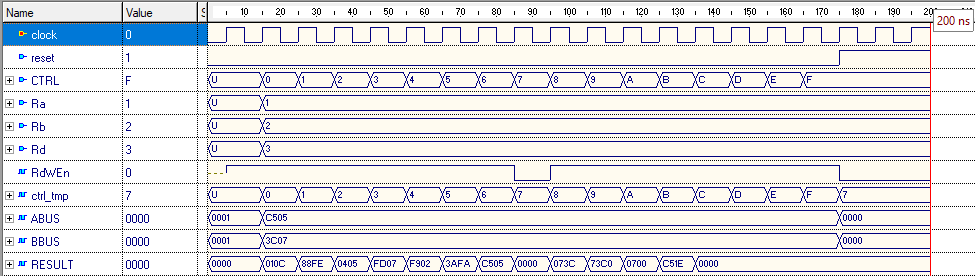
\includegraphics[width=1.1\textwidth]{Top-Level System Simulation.png}
  \caption{Full system simulation waveform --- \texttt{tb\_crypto}
           (Active-HDL capture, 10~ns clock, 200~ns total).}
  \label{fig:sys_wave}
\end{figure}

% ============================================================
\chapter{Conclusion}
% ============================================================

This project has successfully designed, implemented, and simulated a
\textbf{16-bit Cryptographic Coprocessor (CryptoCore-16)} in VHDL,
demonstrating the viability and advantages of hardware-based cryptographic
acceleration over software-only approaches.

\subsection*{Key Achievements}

\begin{enumerate}[label=\arabic*.]
  \item \textbf{Modular Architecture:} The design is structured into five
        self-contained, independently testable VHDL entities: the Register File,
        the ALU, the Shifter, the LUT (S-Box), and the Combinational Logic Block.
        This modularity facilitates debugging, unit testing, and future expansion.

  \item \textbf{Complete 12-Instruction ISA:} The coprocessor supports 12 distinct
        instructions across three functional unit classes—arithmetic/logic (ALU),
        bit manipulation (Shifter), and non-linear substitution (LUT)—encoded
        compactly in a 4-bit opcode field.

  \item \textbf{Correct Functional Behaviour:} All six VHDL testbenches confirmed
        that every component and the full system produce correct outputs for all
        tested input combinations, including boundary conditions (zero operands,
        NOP, reset, and all 256 S-Box inputs).

  \item \textbf{Parallel Execution:} By computing ALU, Shifter, and LUT results
        simultaneously in every clock cycle and using a control MUX to route the
        relevant output, the design achieves a throughput of one instruction per
        clock cycle for all operations.

  \item \textbf{Constant-Time S-Box:} The nibble-based LUT implementation evaluates
        in a single combinational pass with no data-dependent timing, offering
        inherent resistance to timing side-channel attacks.

  \item \textbf{Synthesisable VHDL:} The design uses only synthesisable constructs, including
        \texttt{ieee.std\_logic\_1164}, \texttt{ieee.numeric\_std}, concurrent statements,
        sequential statements, and structural port maps, so it is suitable for direct
        synthesis and deployment on an FPGA target.
\end{enumerate}

\subsection*{Performance Summary}

\begin{itemize}
  \item \textbf{Throughput:} 1 instruction per clock cycle (after the first pipeline stage).
  \item \textbf{Pipeline depth:} 1 stage (input register → combinational logic → write-back).
  \item \textbf{Data width:} 16 bits across all datapaths.
  \item \textbf{Register file:} 16 $\times$ 16-bit registers (256 bits total).
  \item \textbf{S-Box latency:} Single combinational evaluation (zero-cycle).
\end{itemize}

\subsection*{Future Work}

Potential enhancements to the current design include:

\begin{itemize}
  \item Expanding the data path to 32 or 128 bits to support full AES block encryption.
  \item Adding an Inverse S-Box (Inv-S-Box) for decryption support.
  \item Implementing a Linear Feedback Shift Register (LFSR) to provide
        pseudo-random number generation for key scheduling.
  \item Integrating a carry/zero/overflow flags register for conditional branching.
\end{itemize}

% ============================================================
%   REFERENCES
% ============================================================
\begin{thebibliography}{99}

\bibitem{tan2021hardware}
D.~T.~B. Kai and C.~Uttraphan,
``Hardware Implementation of a Cryptographic Coprocessor,''
\textit{Evolution in Electrical and Electronic Engineering},
vol.~2, no.~2, pp.~308--317, 2021.
DOI: \href{https://doi.org/10.30880/eeee.2021.02.02.037}{10.30880/eeee.2021.02.02.037}

\bibitem{nassim2025fpga}
M.~K.~A. Nassim and Z.~Zakarya,
``FPGA-based implementation of an S-Box cryptographic co-processor for high-performance applications,''
\textit{Indonesian Journal of Electrical Engineering and Computer Science},
vol.~40, no.~2, pp.~1167--1176, Nov.~2025.
DOI: \href{https://doi.org/10.11591/ijeecs.v40.i2.pp1167-1176}{10.11591/ijeecs.v40.i2.pp1167-1176}

\bibitem{fpga4student}
FPGA4Student,
``Cryptographic Coprocessor Design in VHDL,''
[Online]. Available:
\url{https://www.fpga4student.com/2017/07/cryptographic-coprocessor-design-in-vhdl.html}
[Accessed: Apr.~2026].


\bibitem{joshi2014vhdl}
R.~Joshi, N.~Naik, N.~Kashid, S.~Waykar, and C.~Rangrass,
``VHDL implementation of 16-bit ALU,''
\textit{International Journal of Engineering Research and Technology},
vol.~2, no.~4, pp.~1--4, 2014.
DOI: \href{https://doi.org/10.17577/IJERTCONV2IS04050}{10.17577/IJERTCONV2IS04050}

\bibitem{patel2023fpga}
S.~Patel and R.~Kumar,
``Educational use of FPGA boards in computer engineering,''
\textit{International Journal of Engineering Education},
vol.~39, no.~4, pp.~1247--1260, 2023.

\bibitem{hamzah2017aes}
H.~Hamzah, N.~Ahmad, M.~H.~Jabbar, and C.~F.~Soon,
``Optimization AES S-Box/Inv S-Box using FPGA implementation,''
\textit{Journal of Telecommunication, Electronic and Computer Engineering (JTEC)},
vol.~9, no.~3--8, pp.~133--136, 2017.

\bibitem{anwar2013fpga}
H.~Anwar, M.~Daneshtalab, M.~Ebrahimi, J.~Plosila, and H.~Tenhunen,
``FPGA implementation of AES-based crypto processor,''
in \textit{Proc. IEEE International Conference on Electronics, Circuits, and Systems},
Dec.~2013, pp.~369--372.
DOI: \href{https://doi.org/10.1109/ICECS.2013.6815431}{10.1109/ICECS.2013.6815431}

\bibitem{kumar2021aes}
T.~M. Kumar \textit{et al.},
``A low area high speed FPGA implementation of AES architecture for cryptography application,''
\textit{Electronics (Switzerland)},
vol.~10, no.~16, p.~2023, Aug.~2021.
DOI: \href{https://doi.org/10.3390/electronics10162023}{10.3390/electronics10162023}



\bibitem{haroldo2024dynamic}
C.~M. Haroldo, N.~C. David, M.~Madani, and E.~B. Bourennane,
``FPGA implementation of AES-based on optimized dynamic S-Box,''
in \textit{Proc. International Conference on Security and Cryptography},
2024, pp.~730--737.
DOI: \href{https://doi.org/10.5220/0012780300003767}{10.5220/0012780300003767}


\end{thebibliography}

\end{document}